




% Linke Hälfte der A3-Seite
%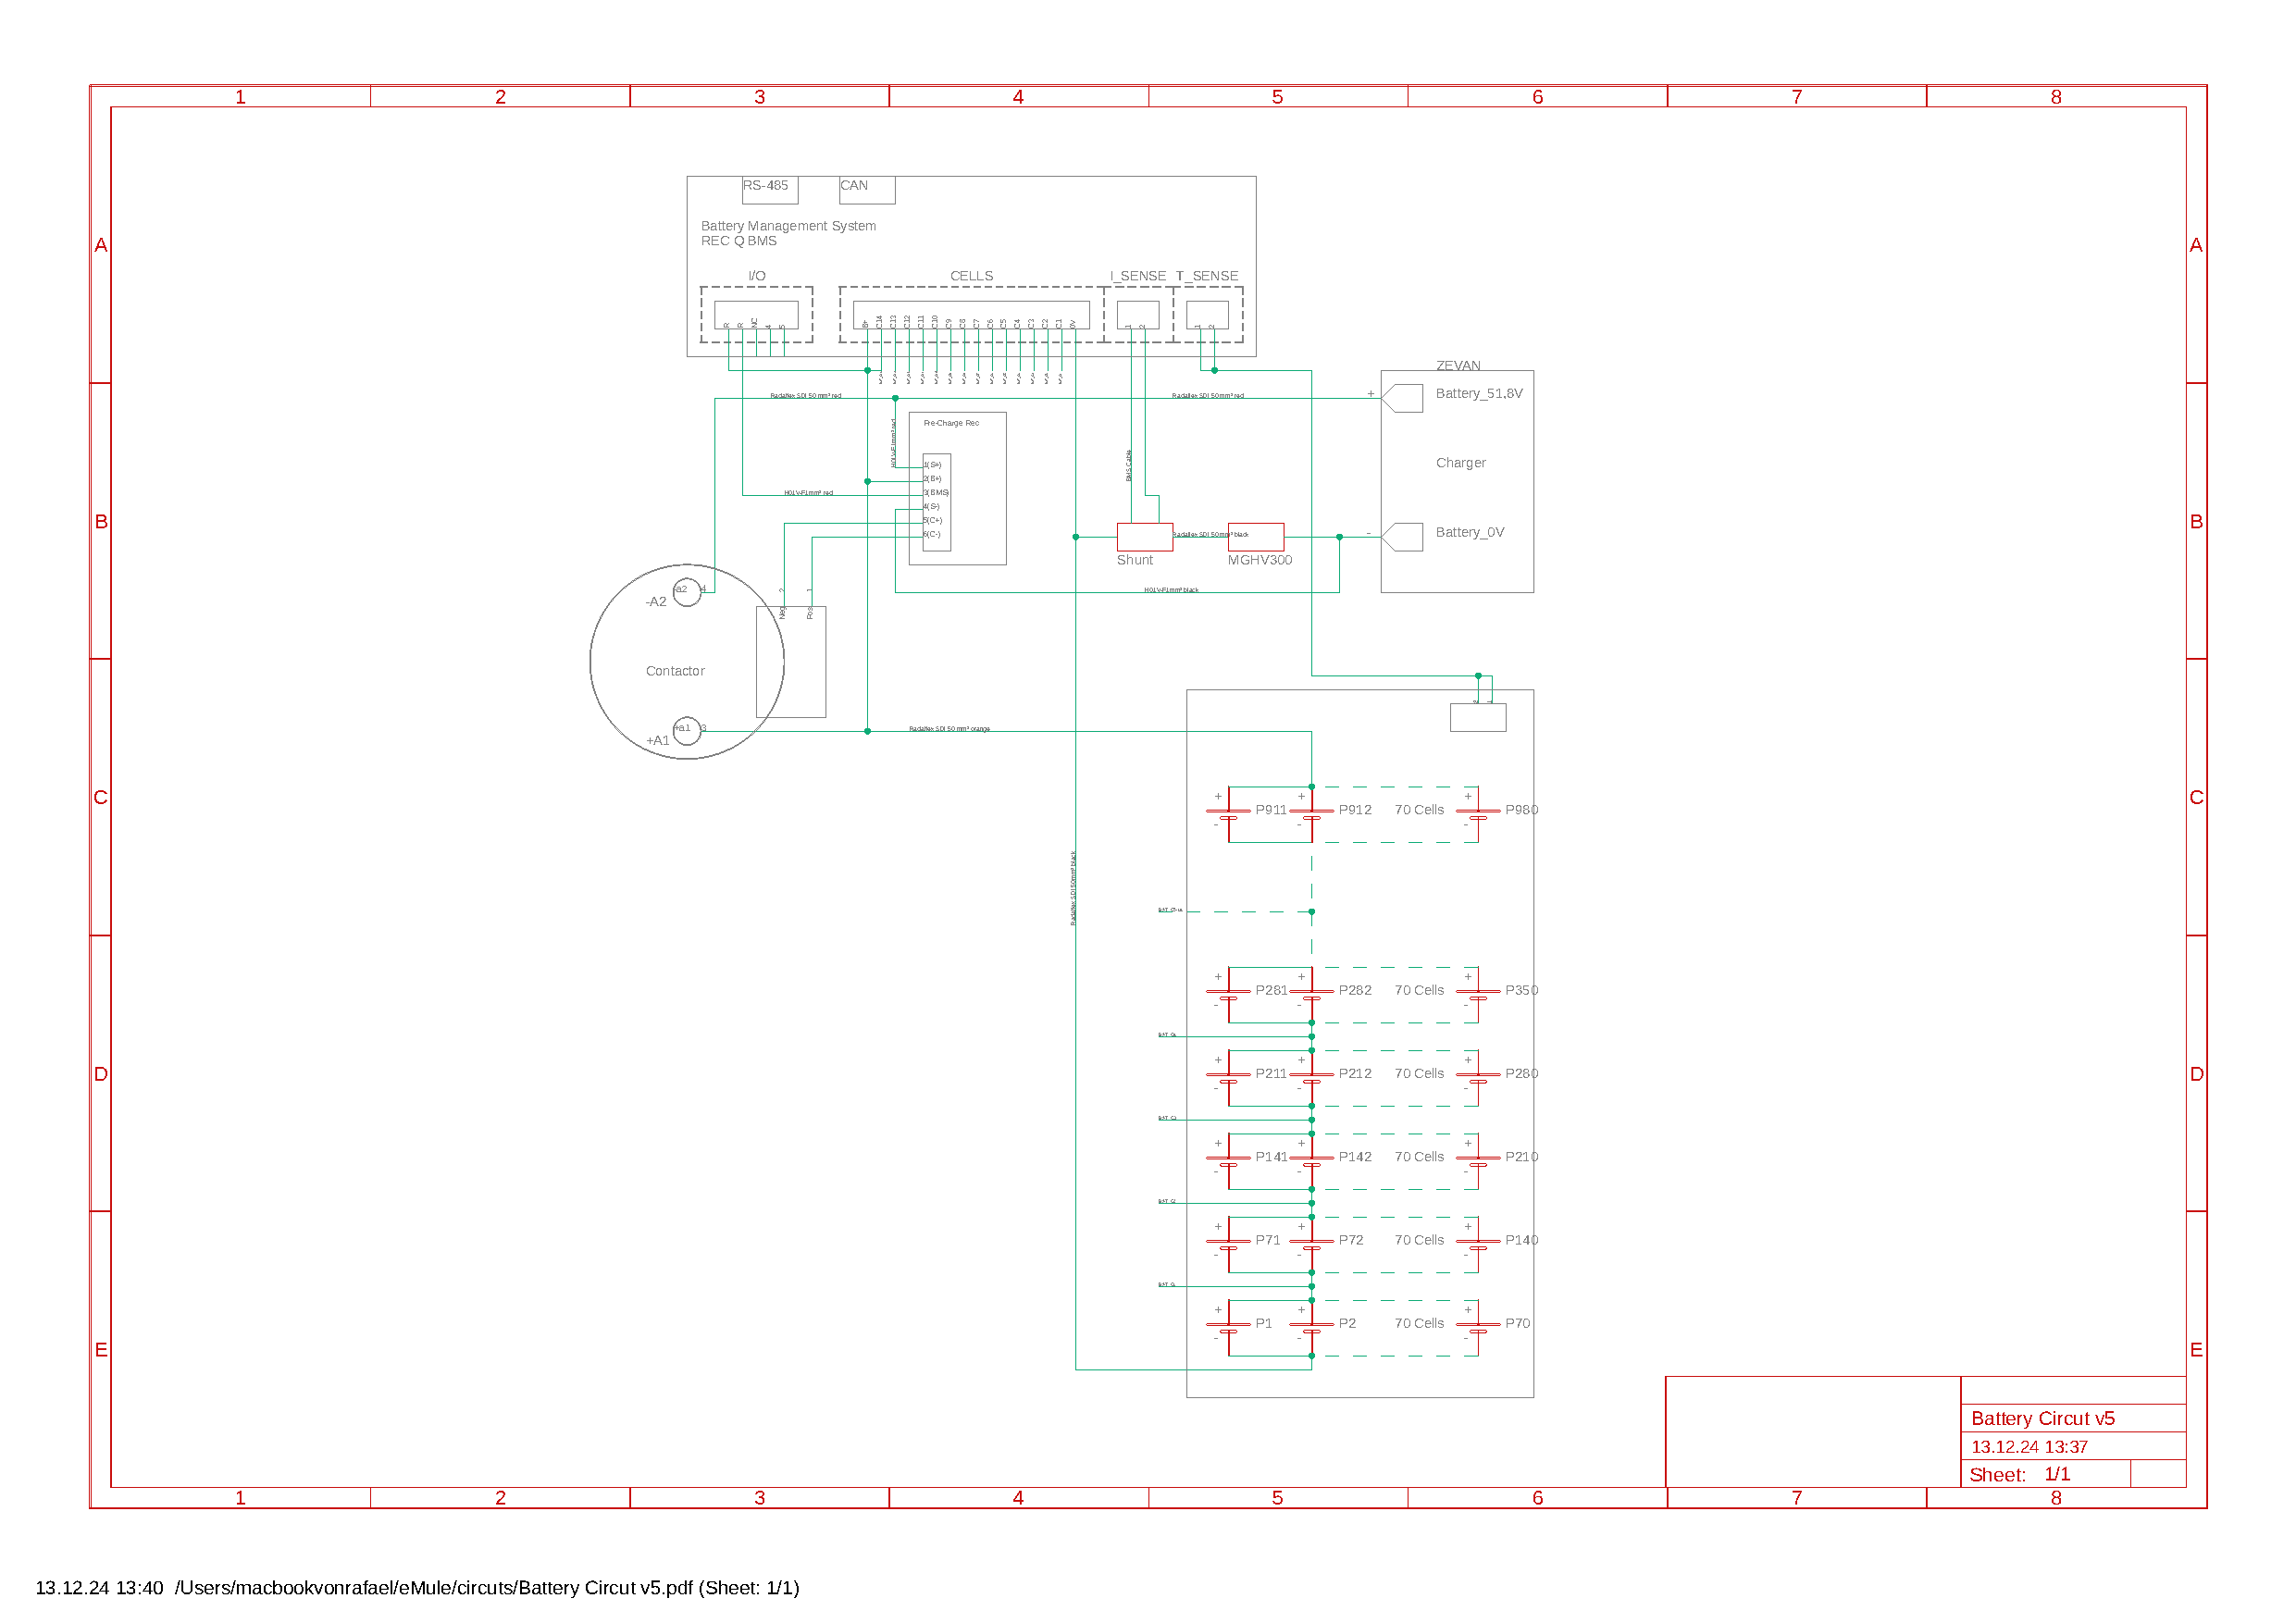
\includepdf[pages=1, trim=0cm 0cm 21cm 0cm, clip]{circuts/Battery Circut v5.pdf}

% Rechte Hälfte der A3-Seite
%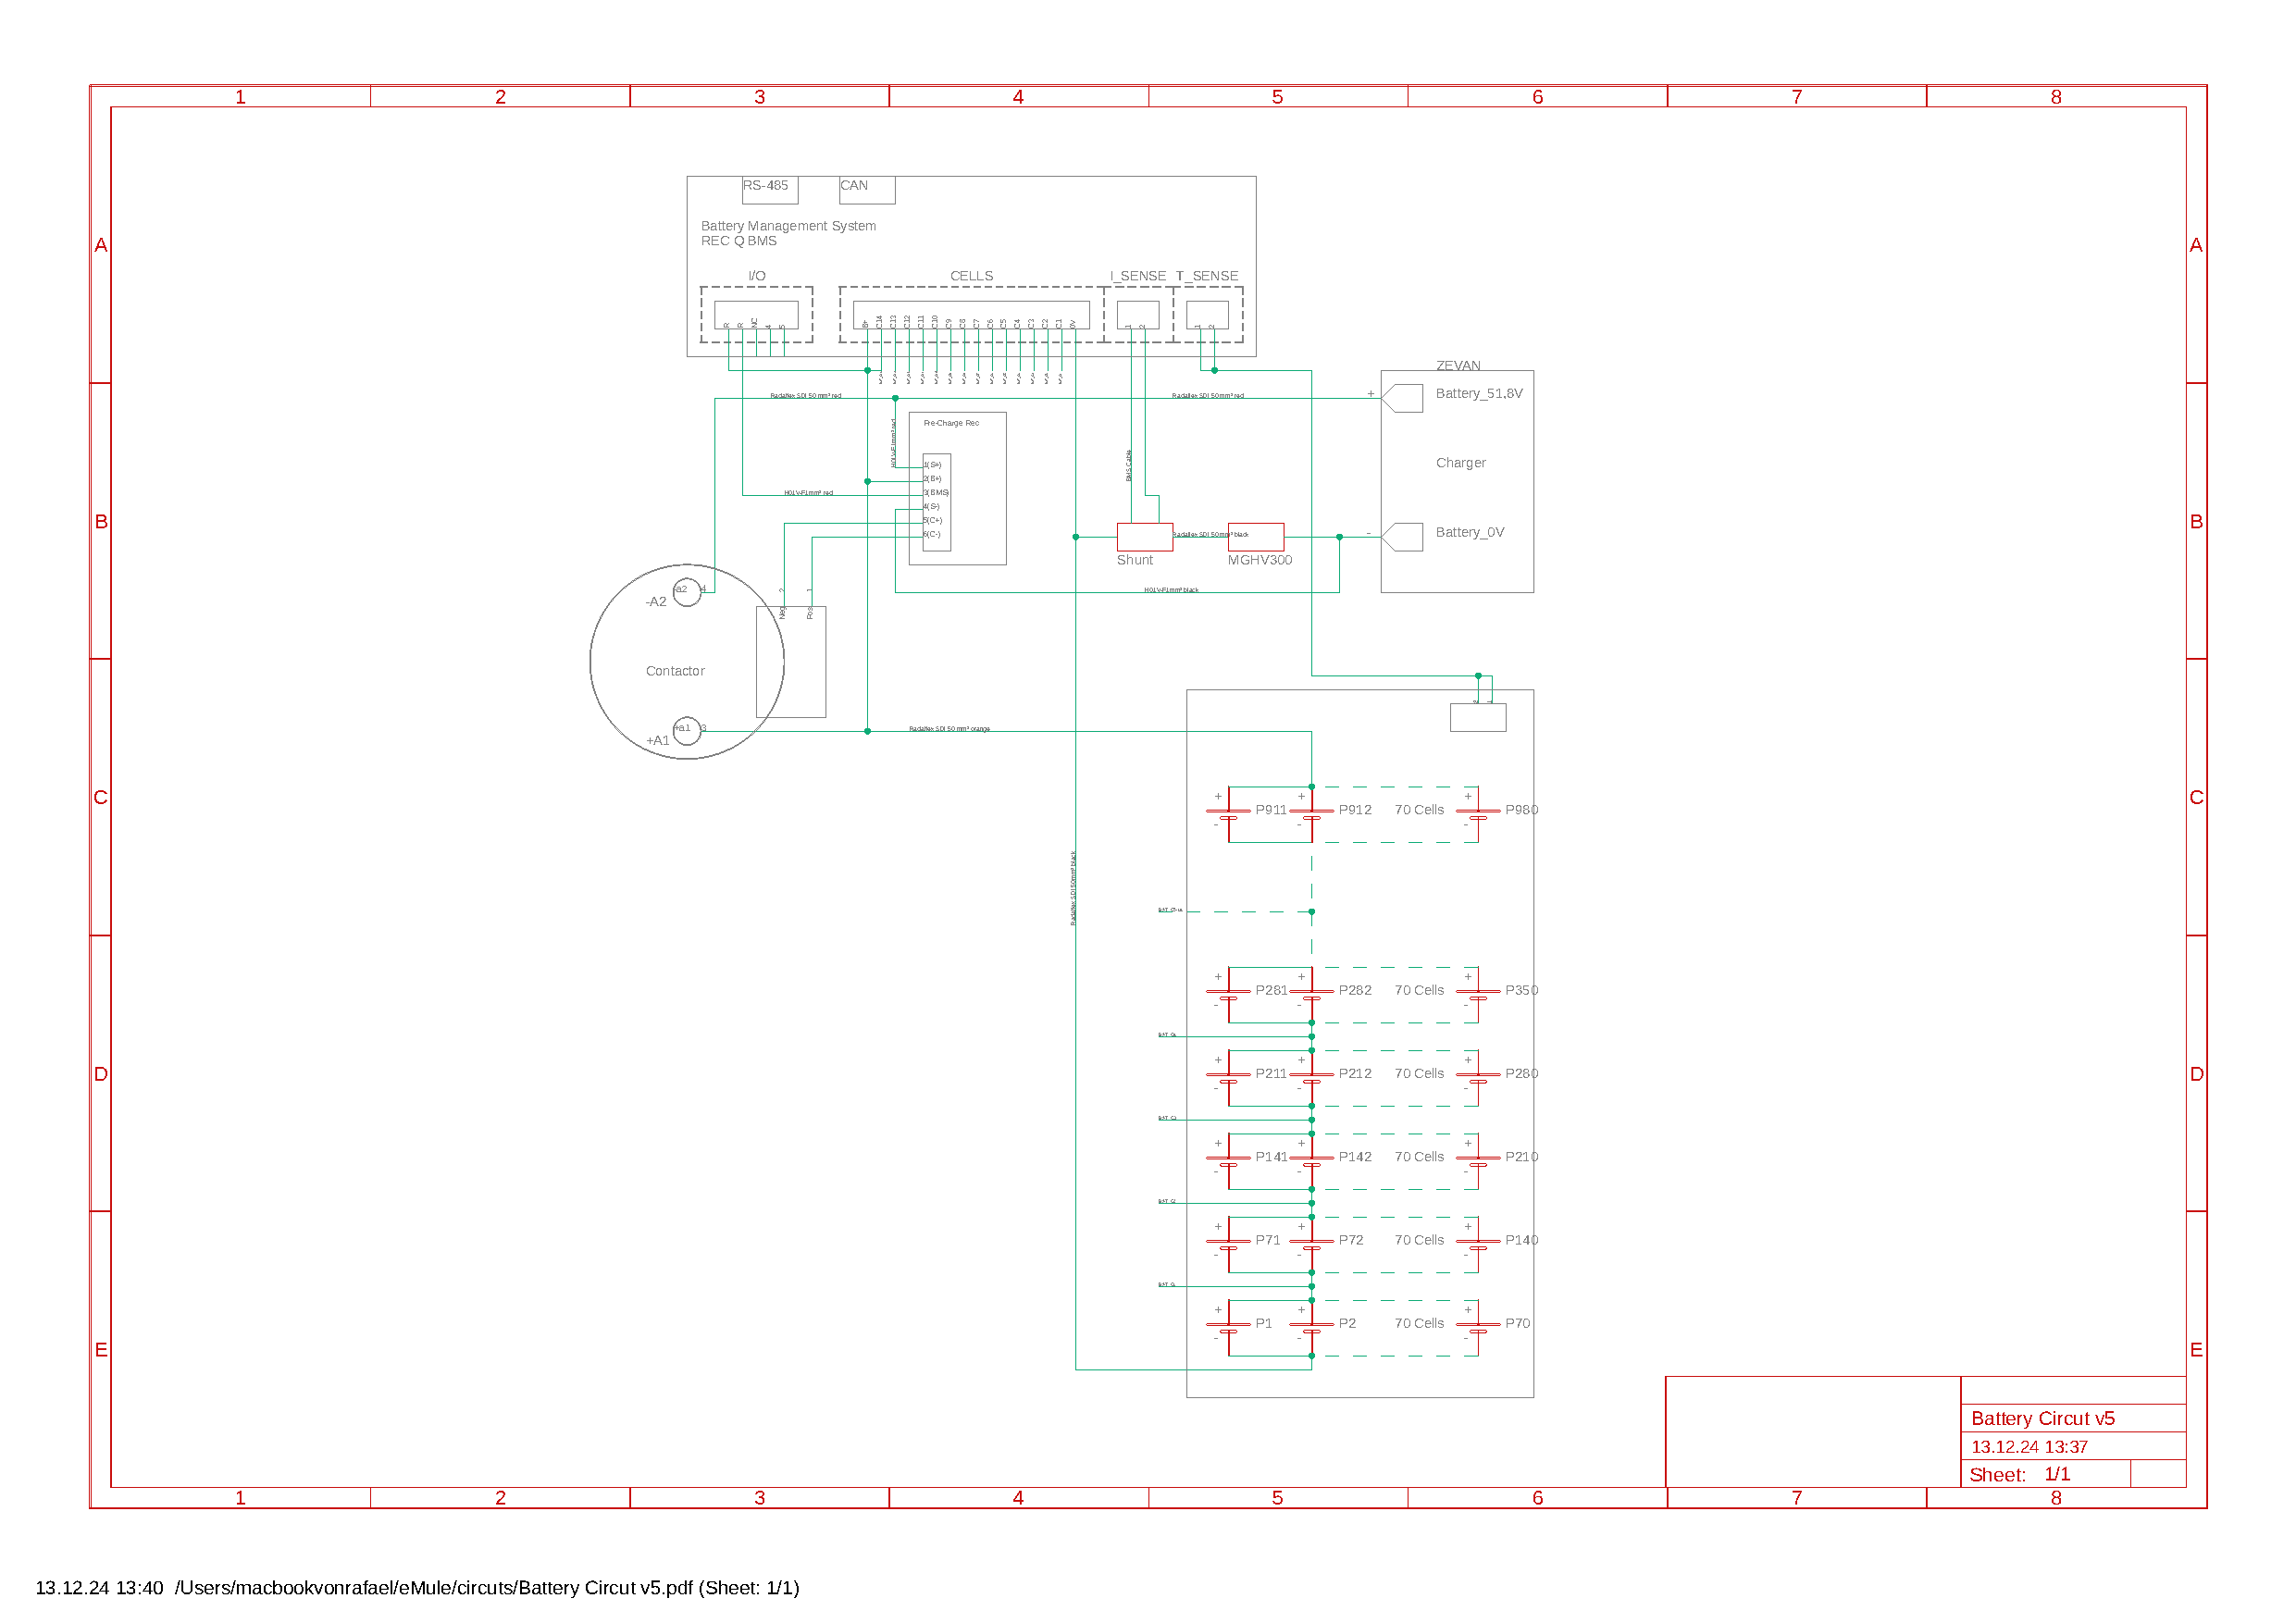
\includepdf[pages=1, trim=21cm 0cm 0cm 0cm, clip]{circuts/Battery Circut v5.pdf}

%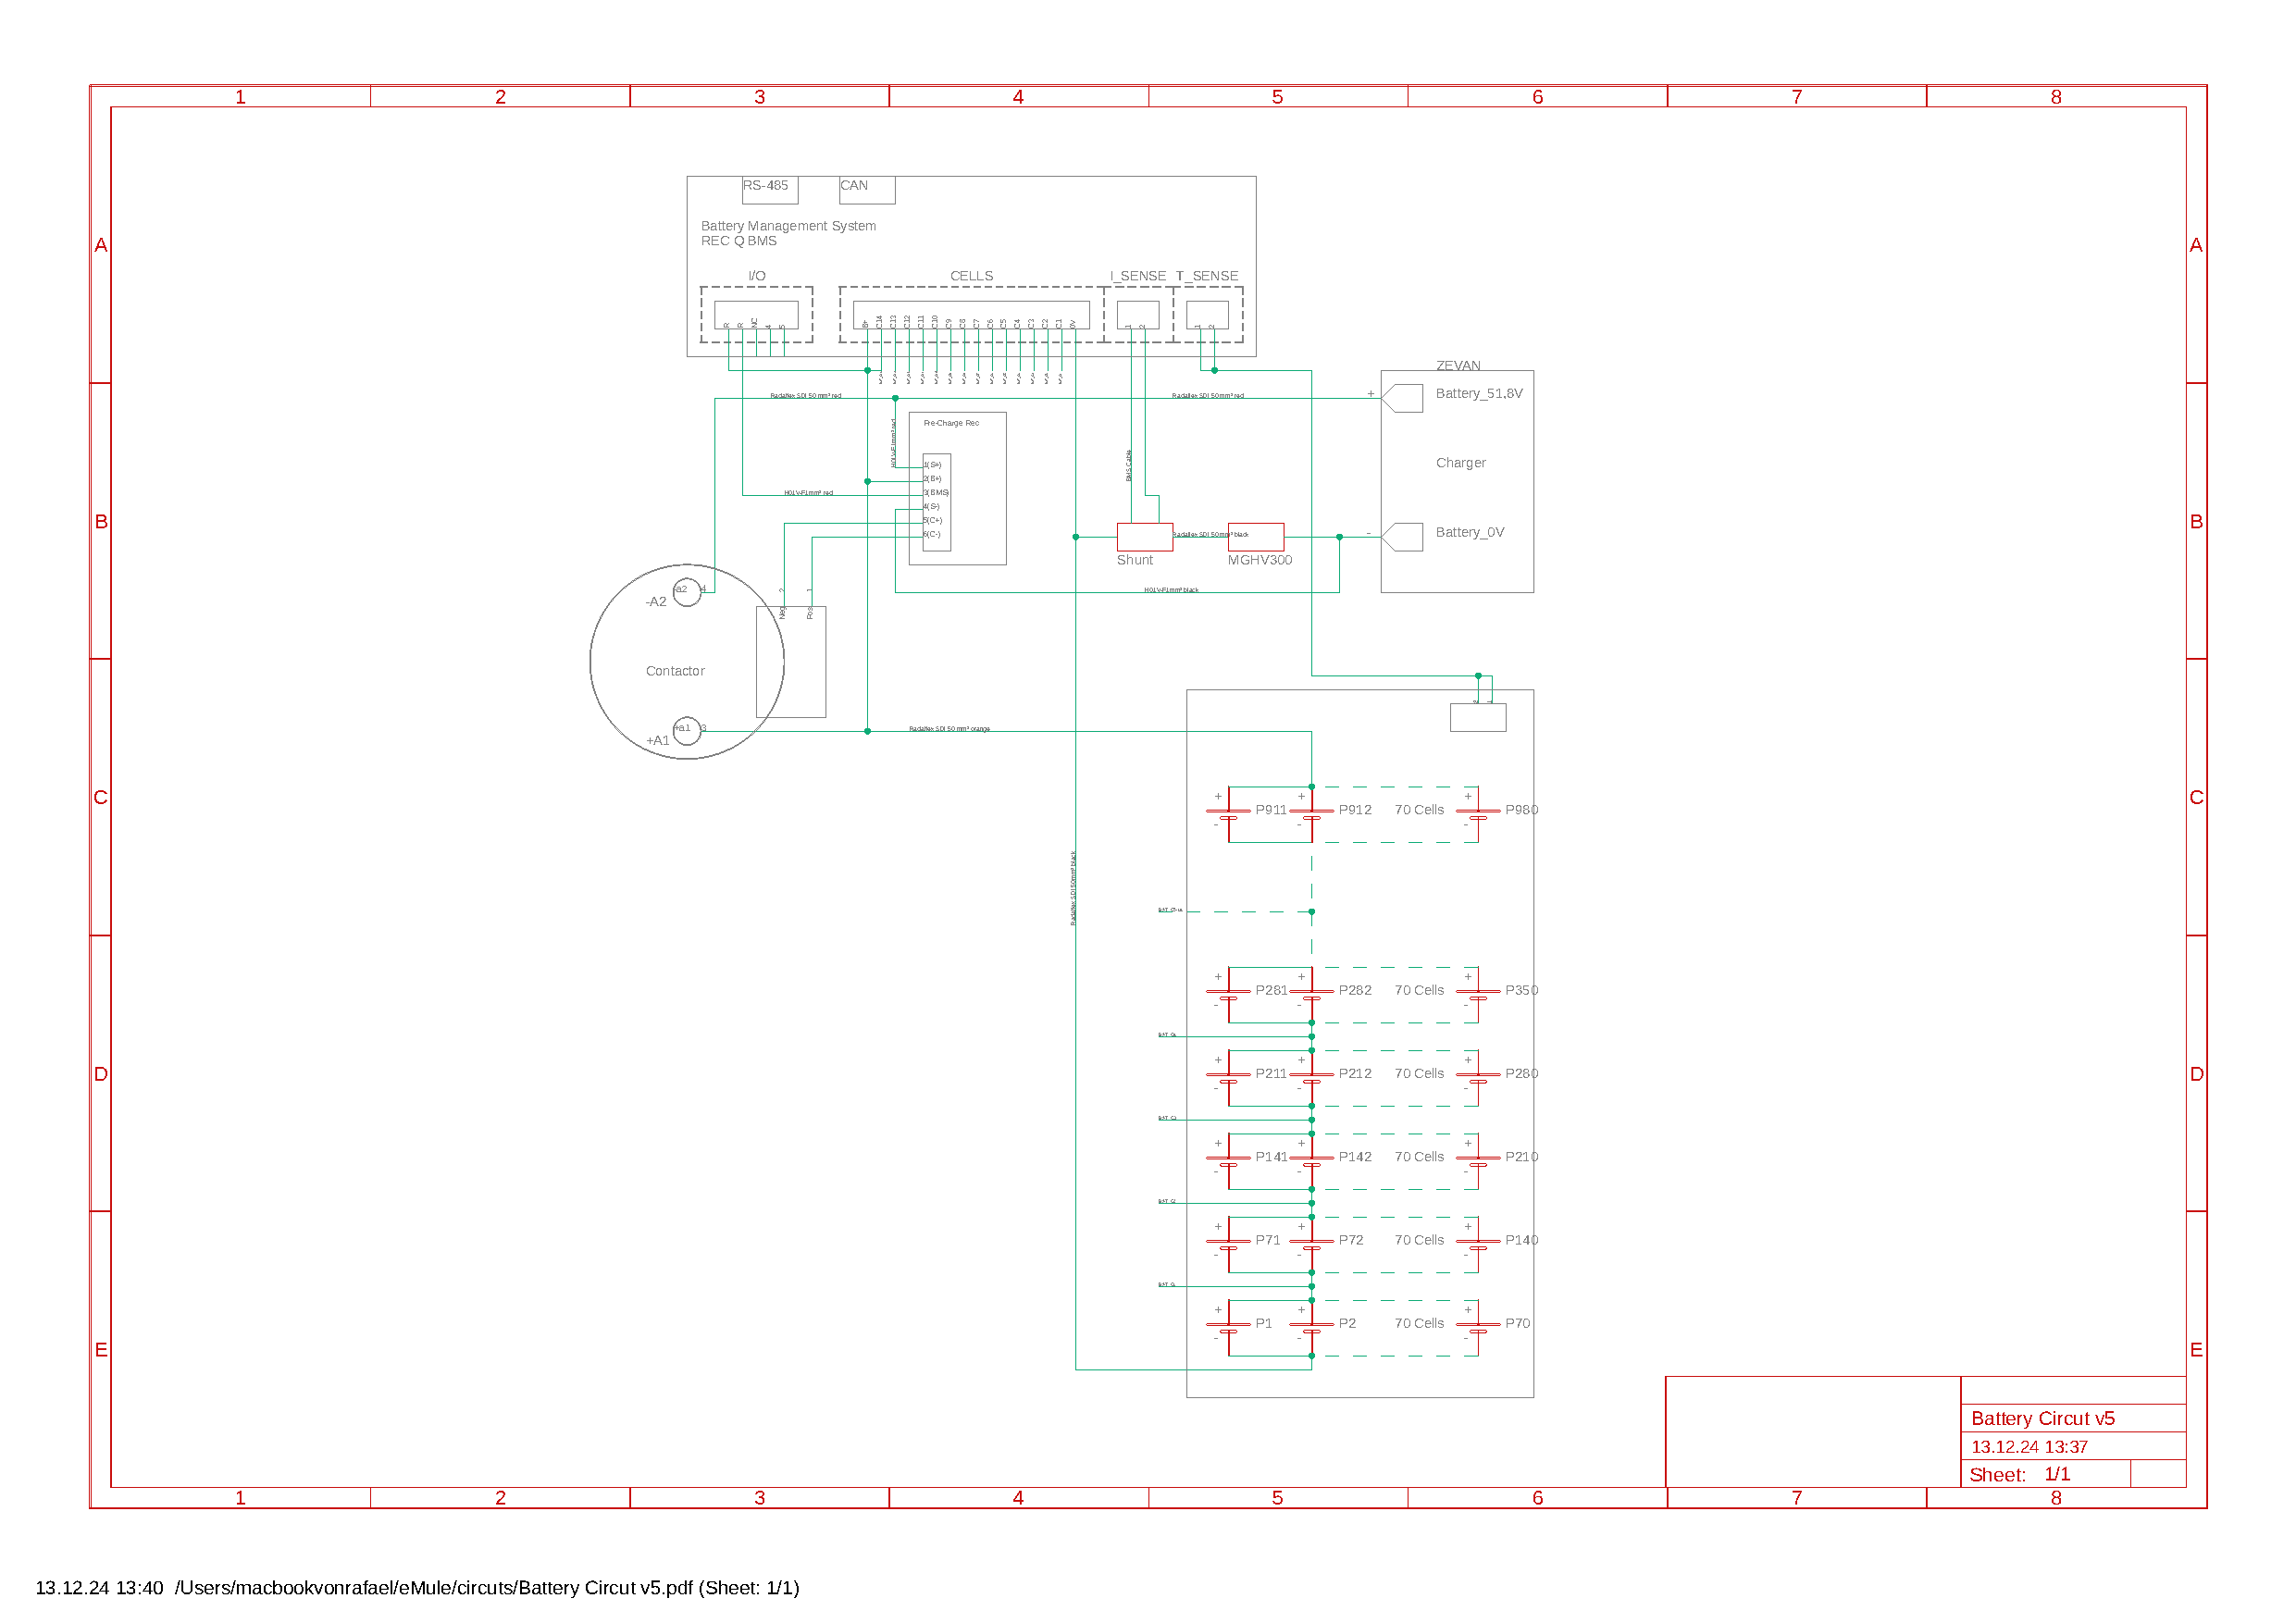
\includepdf[pages=1, angle=90, fitpaper=true]{circuts/Battery Circut v5.pdf}
\section{Stromlaufpläne}
\subsection{Stromlaufplan Battery Circuit}
Für die Erstellung des \textit{Battery Circuit} (siehe Abbildung \ref{fig:battery_circuit}) Stromlaufplans nach festgelegter Norm und aktuellem Verbaustand wird der vorliegende Plan zunächst ausgedruckt. Im ersten Schritt wird dieser Stromlaufplan systematisch auf Unstimmigkeiten, wie fehlende Verbindungen oder unklare Symbolik, überprüft. Gefundene Fehler werden im nächsten Schritt markiert und anschließend korrigiert, wobei die Einhaltung elektrotechnischer Standards gewährleistet wird. Zudem erfolgt eine Layoutanpassung zur Verbesserung der Übersichtlichkeit. Im letzten Schritt muss herausgefunden werden, nach welcher Norm der Stromlaufplan erstellt wurde. Diese Norm muss recherchiert und in die von uns gewählte DIN EN 60617 Norm \glqq übersetzt\grqq {} werden. Der überarbeitete Stromlaufplan wird abschließend mit Autodesk Fusion 360 in ein DIN-A3-Format übertragen. Dabei werden Titelblock und Legende integriert, um die Professionalität und Lesbarkeit sicherzustellen.

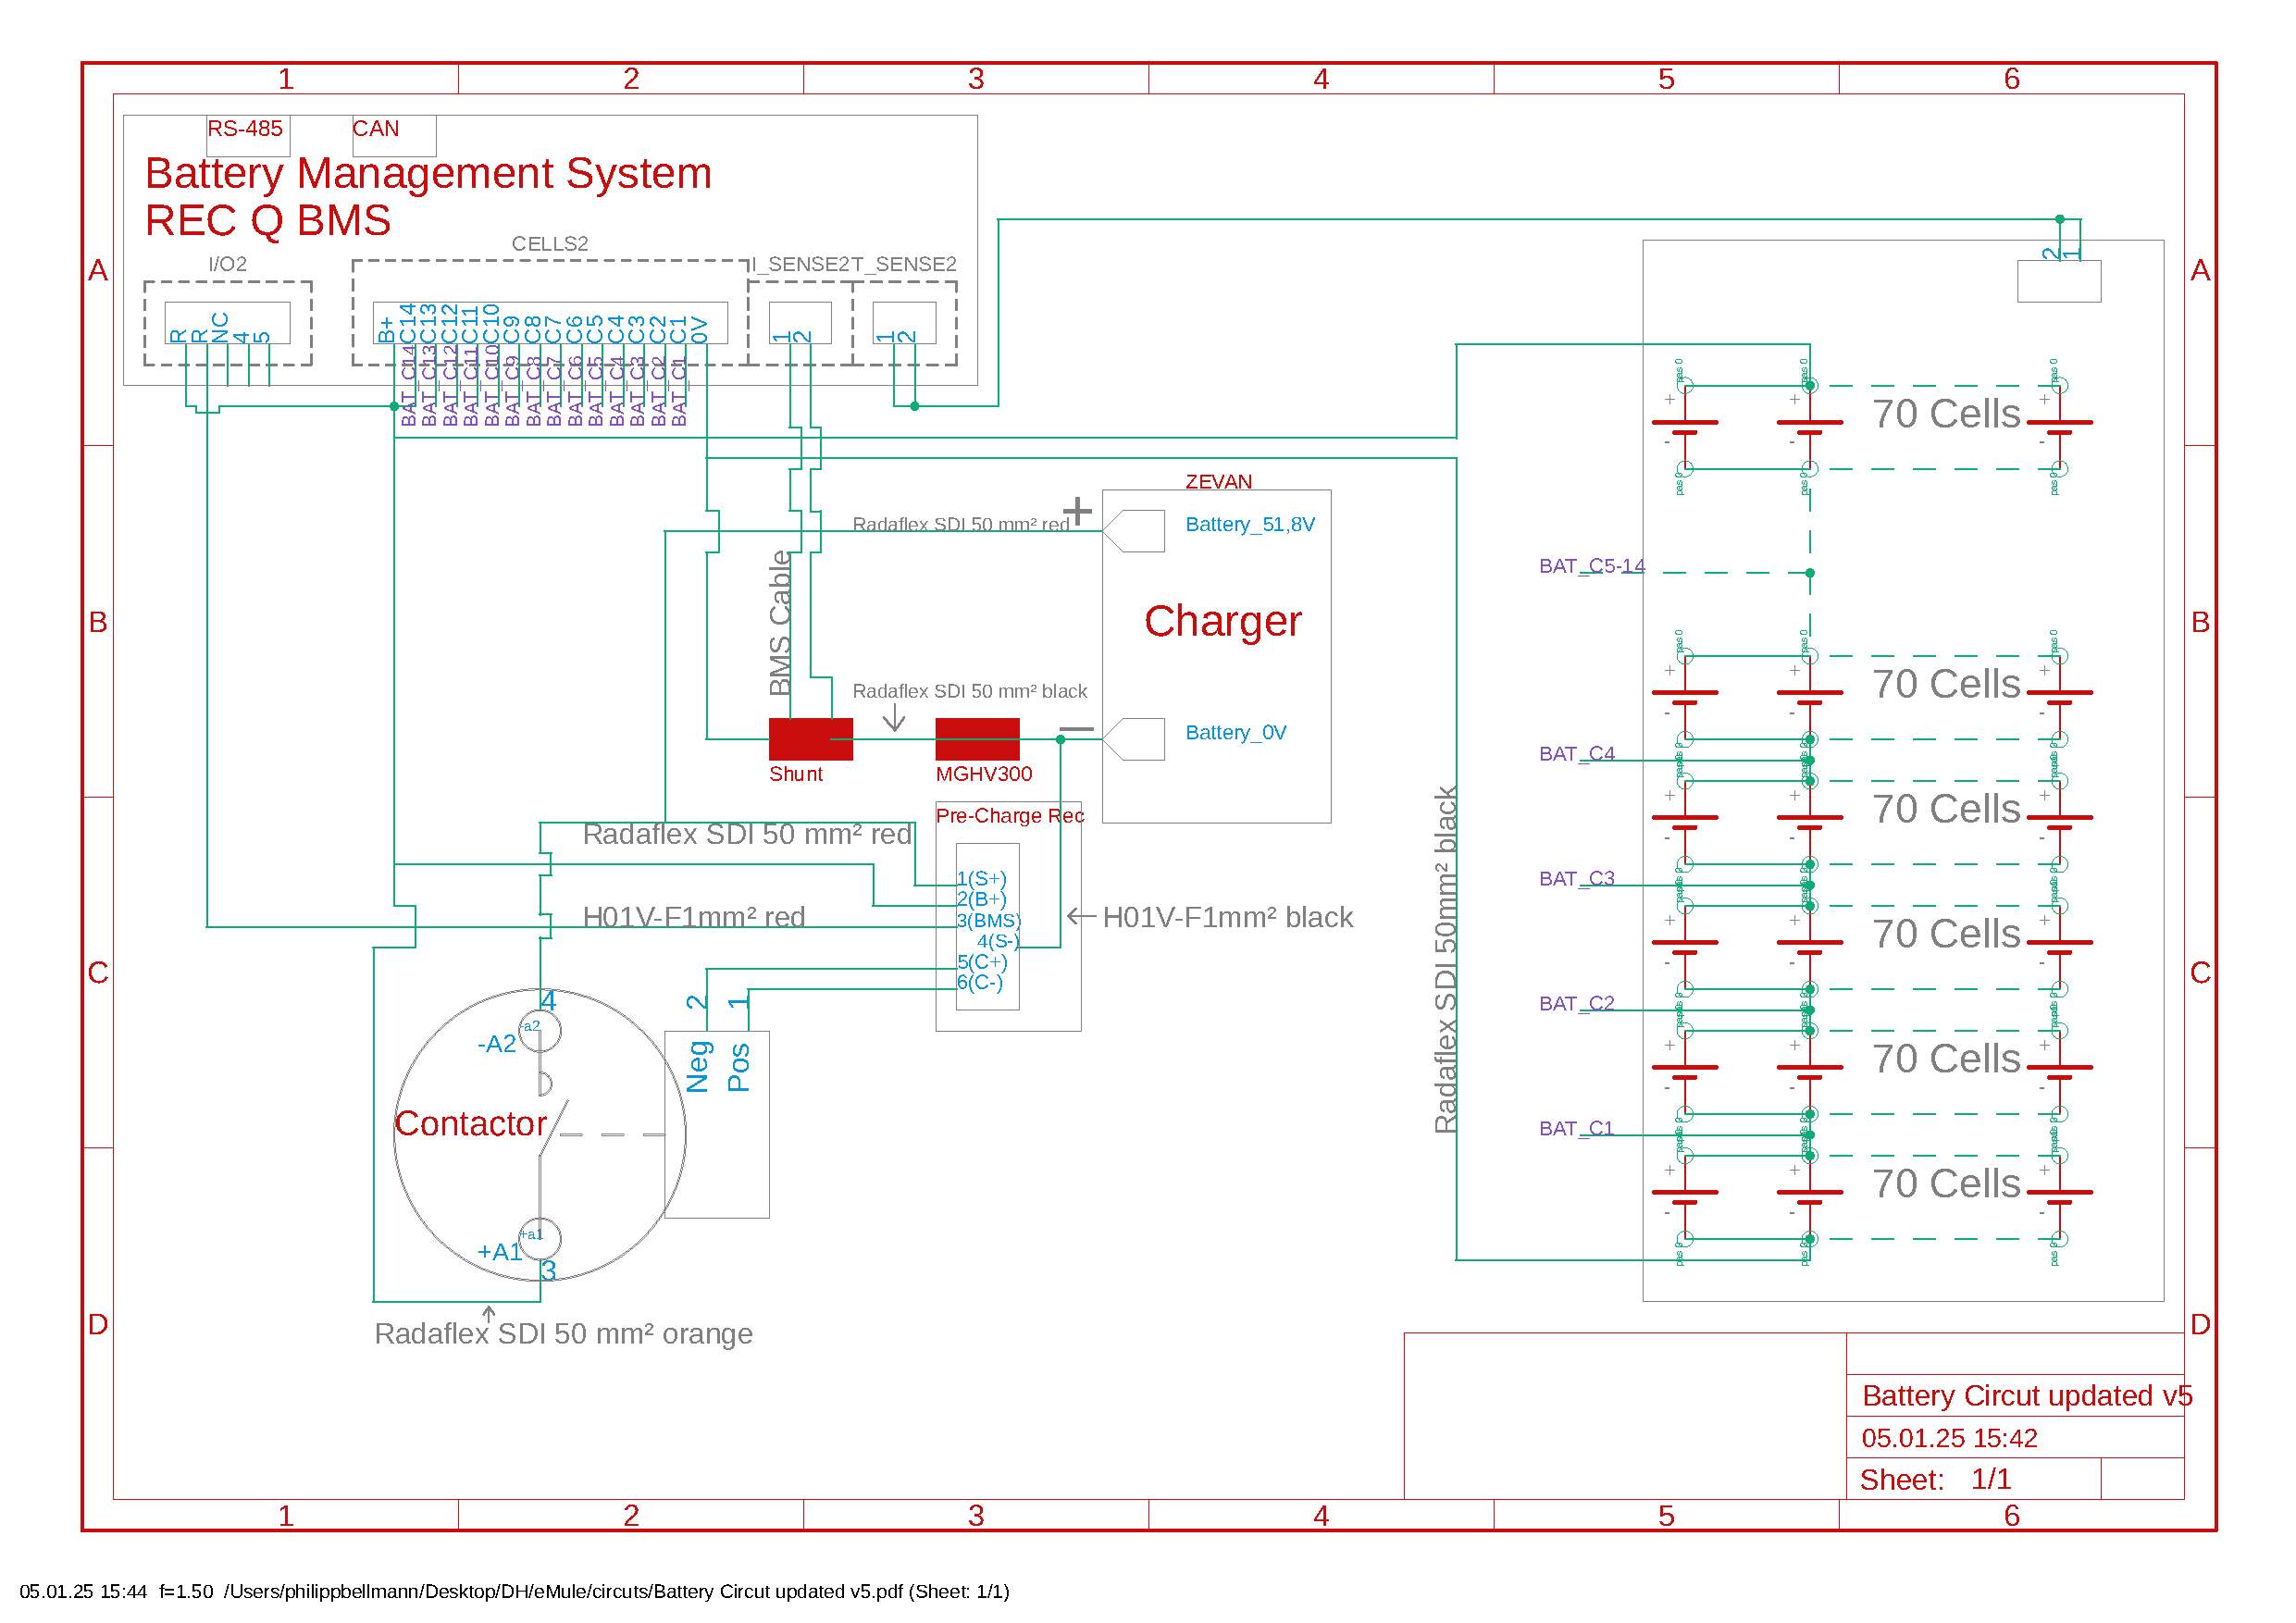
\includepdf[pages=1, fitpaper=true, pagecommand={%
	\thispagestyle{empty} % Entfernt Seitenzahlen und Kopfzeilen
	\begin{center}
		\vspace*{-5cm} % Verschiebt die Caption um 2 cm nach oben
		\hspace{10cm} % Verschiebt die Caption um 10 cm nach rechts
		\captionof{figure}{Schaltplan des Battery Circuits} % Fügt die Caption ein
		\label{fig:battery_circuit} % Für Querverweise
	\end{center}
}]{circuts/Battery Circut updated.pdf}
\addtocounter{page}{1} % Seitenzähler korrekt erhöhen

% Zweite PDF: Motor Controller
\subsection{Stromlaufplan Motor Controller}
Für die Erstellung des \textit{Motor Controller} (siehe Abbildung \ref{fig:motor_controller}) Stromlaufplans nach festgelegter Norm und aktuellem Verbaustand wird der vorliegende Plan zunächst ausgedruckt. Im ersten Schritt wird dieser Stromlaufplan systematisch auf Unstimmigkeiten, wie fehlende Verbindungen oder unklare Symbolik, überprüft. Gefundene Fehler werden im nächsten Schritt markiert und anschließend korrigiert, wobei die Einhaltung elektrotechnischer Standards gewährleistet wird. Zudem erfolgt eine Layoutanpassung zur Verbesserung der Übersichtlichkeit. Im letzten Schritt muss herausgefunden werden, nach welcher Norm der Stromlaufplan erstellt wurde. Diese Norm muss recherchiert und in die von uns gewählte DIN EN 60617 Norm \glqq übersetzt\grqq {} werden. Der überarbeitete Stromlaufplan wird abschließend mit Autodesk Fusion 360 in ein DIN-A3-Format übertragen. Dabei werden Titelblock und Legende integriert, um die Professionalität und Lesbarkeit sicherzustellen.

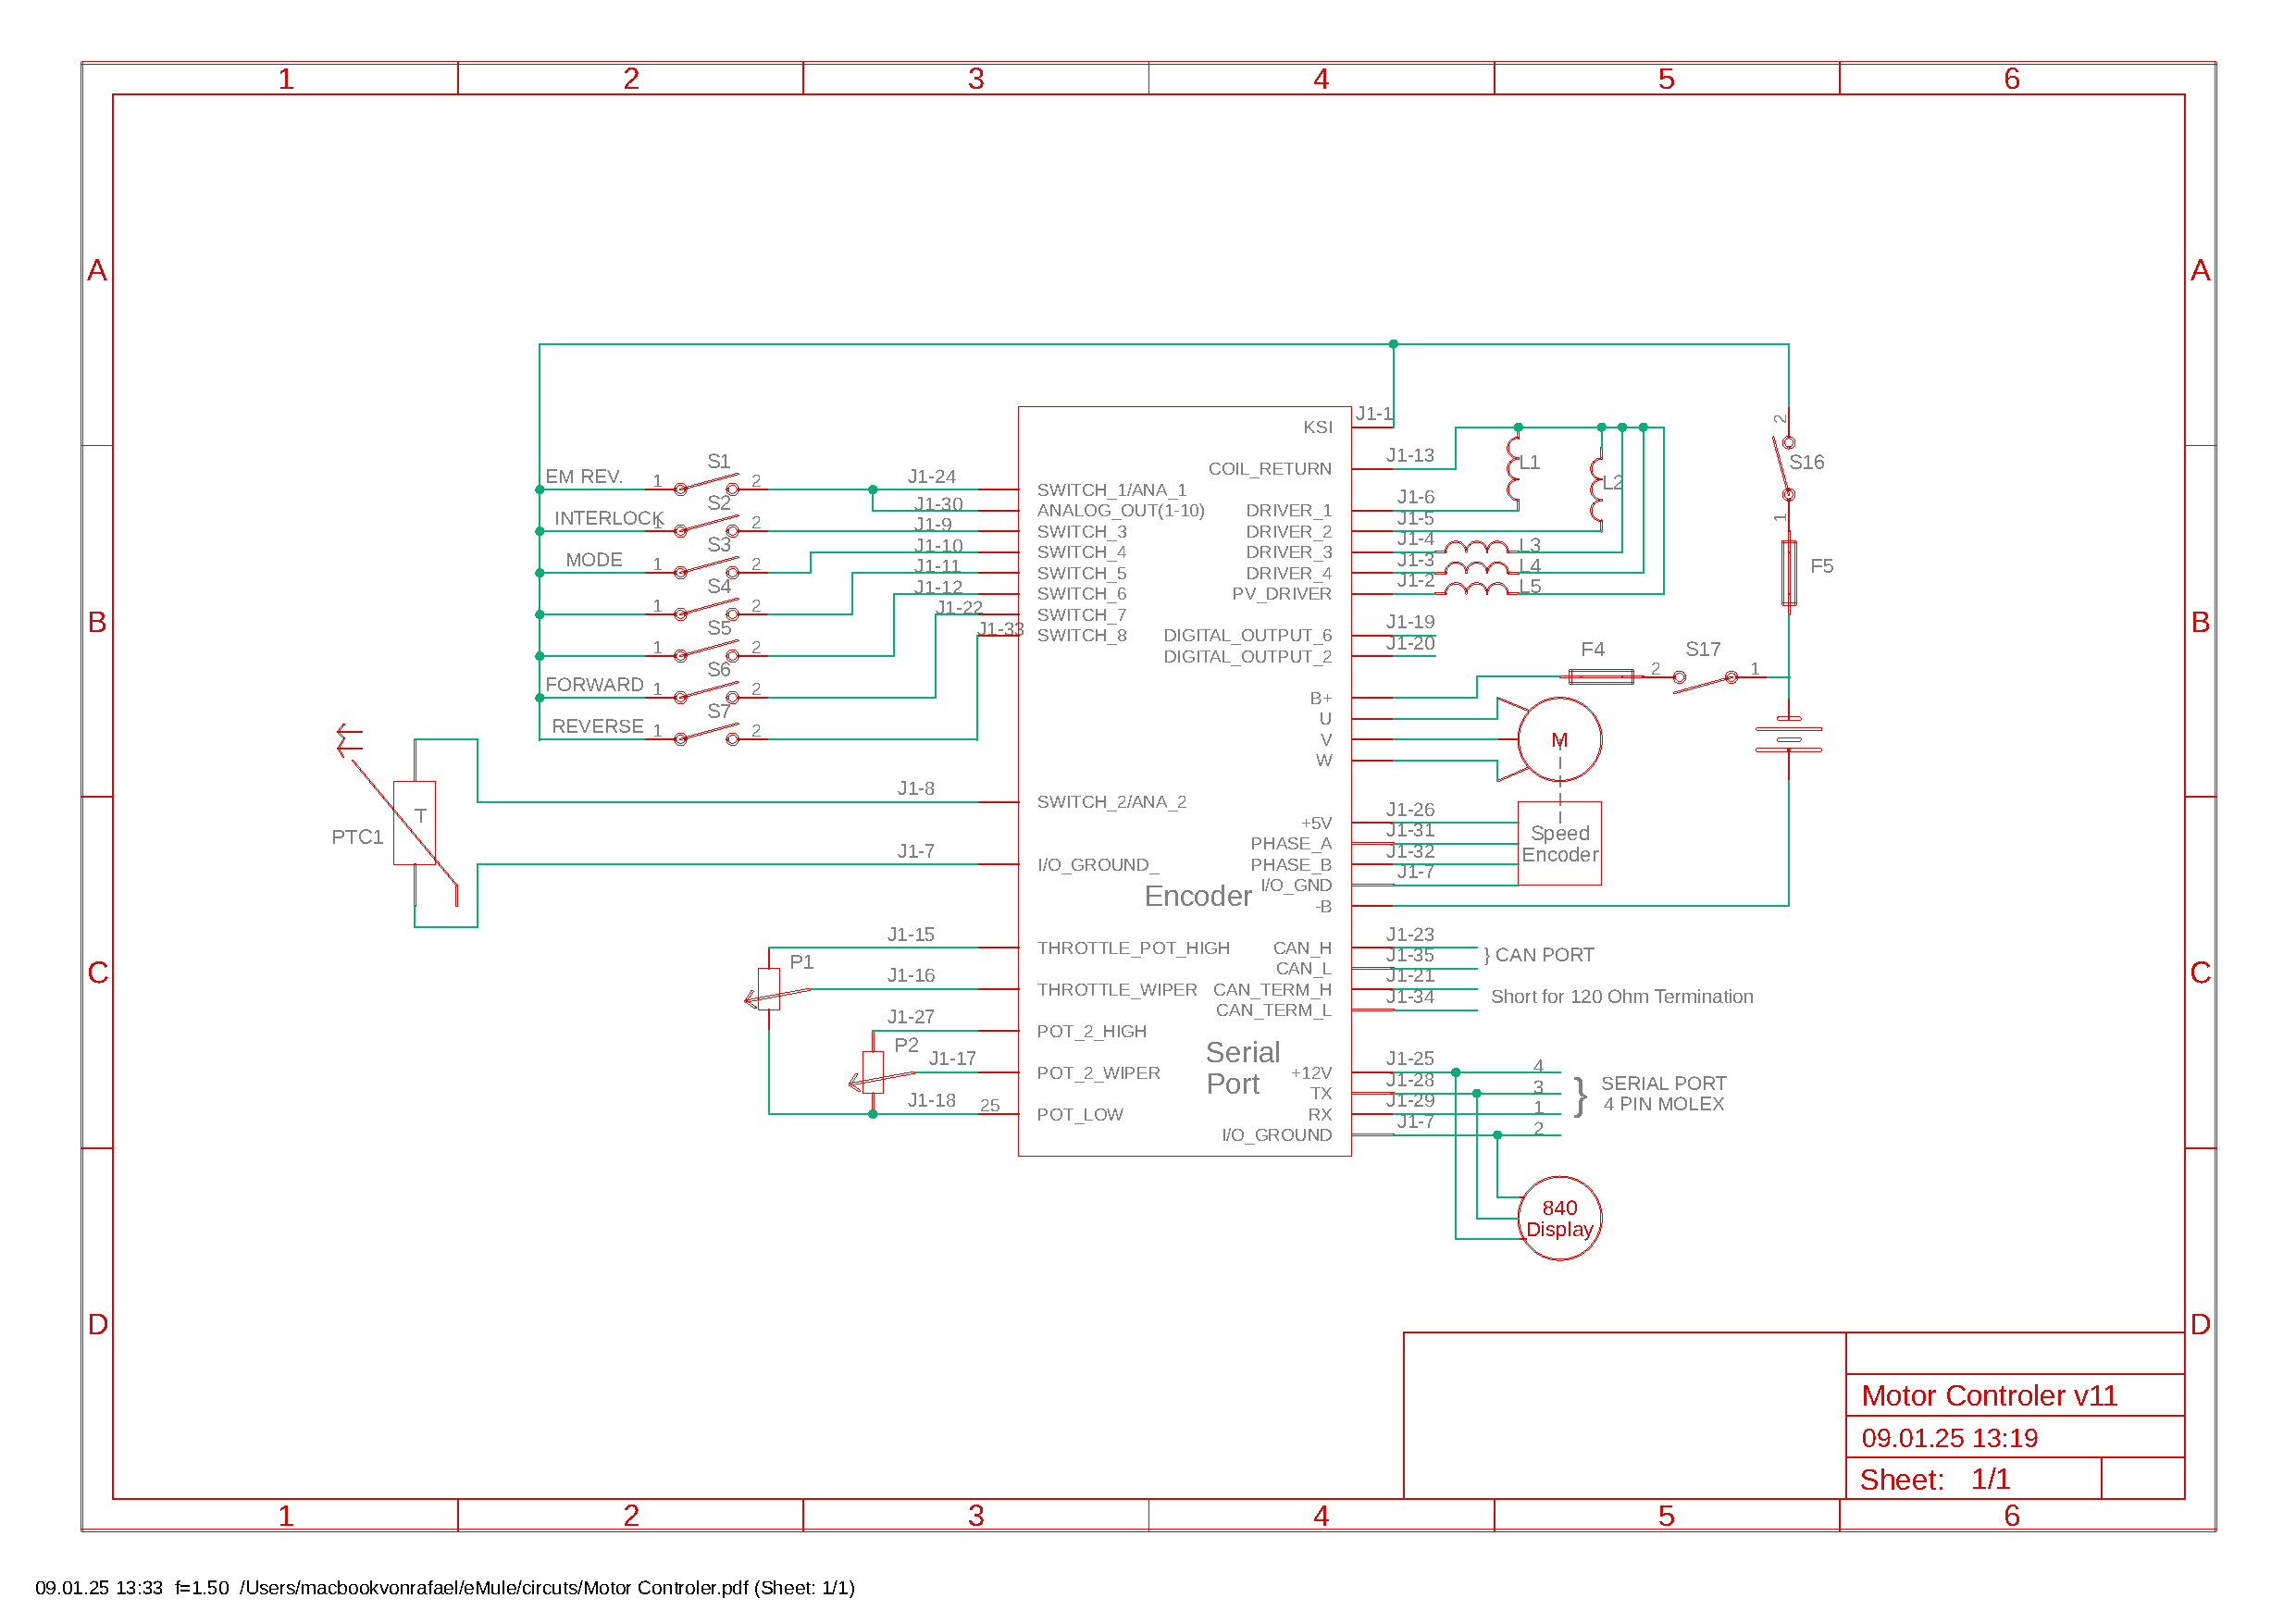
\includepdf[pages=1, fitpaper=true, pagecommand={%
	\thispagestyle{empty} % Entfernt Seitenzahlen und Kopfzeilen
	\begin{center}
		\captionof{figure}{Schaltplan des Motor Controllers} % Fügt die Caption ein
		\label{fig:motor_controller} % Für Querverweise
	\end{center}
}]{circuts/Motor Controler.pdf}
\addtocounter{page}{1} % Seitenzähler korrekt erhöhen

% Dritte PDF: LV-Onboard-Network
\subsection{Stromlaufplan LV-Onboard-Netz}
Für die Erstellung des \textit{LV-Onboard-Netz} (siehe Abbildung \ref{fig:lv_onboard_network}) Stromlaufplans nach festgelegter Norm und aktuellem Verbaustand wird der vorliegende Plan zunächst ausgedruckt. Im ersten Schritt wird dieser Stromlaufplan systematisch auf Unstimmigkeiten, wie fehlende Verbindungen oder unklare Symbolik, überprüft. Gefundene Fehler werden im nächsten Schritt markiert und anschließend korrigiert, wobei die Einhaltung elektrotechnischer Standards gewährleistet wird. Zudem erfolgt eine Layoutanpassung zur Verbesserung der Übersichtlichkeit. Im letzten Schritt muss herausgefunden werden, nach welcher Norm der Stromlaufplan erstellt wurde. Diese Norm muss recherchiert und in die von uns gewählte DIN EN 60617 Norm \glqq übersetzt\grqq {} werden. Der überarbeitete Stromlaufplan wird abschließend mit Autodesk Fusion 360 in ein DIN-A3-Format übertragen. Dabei werden Titelblock und Legende integriert, um die Professionalität und Lesbarkeit sicherzustellen.

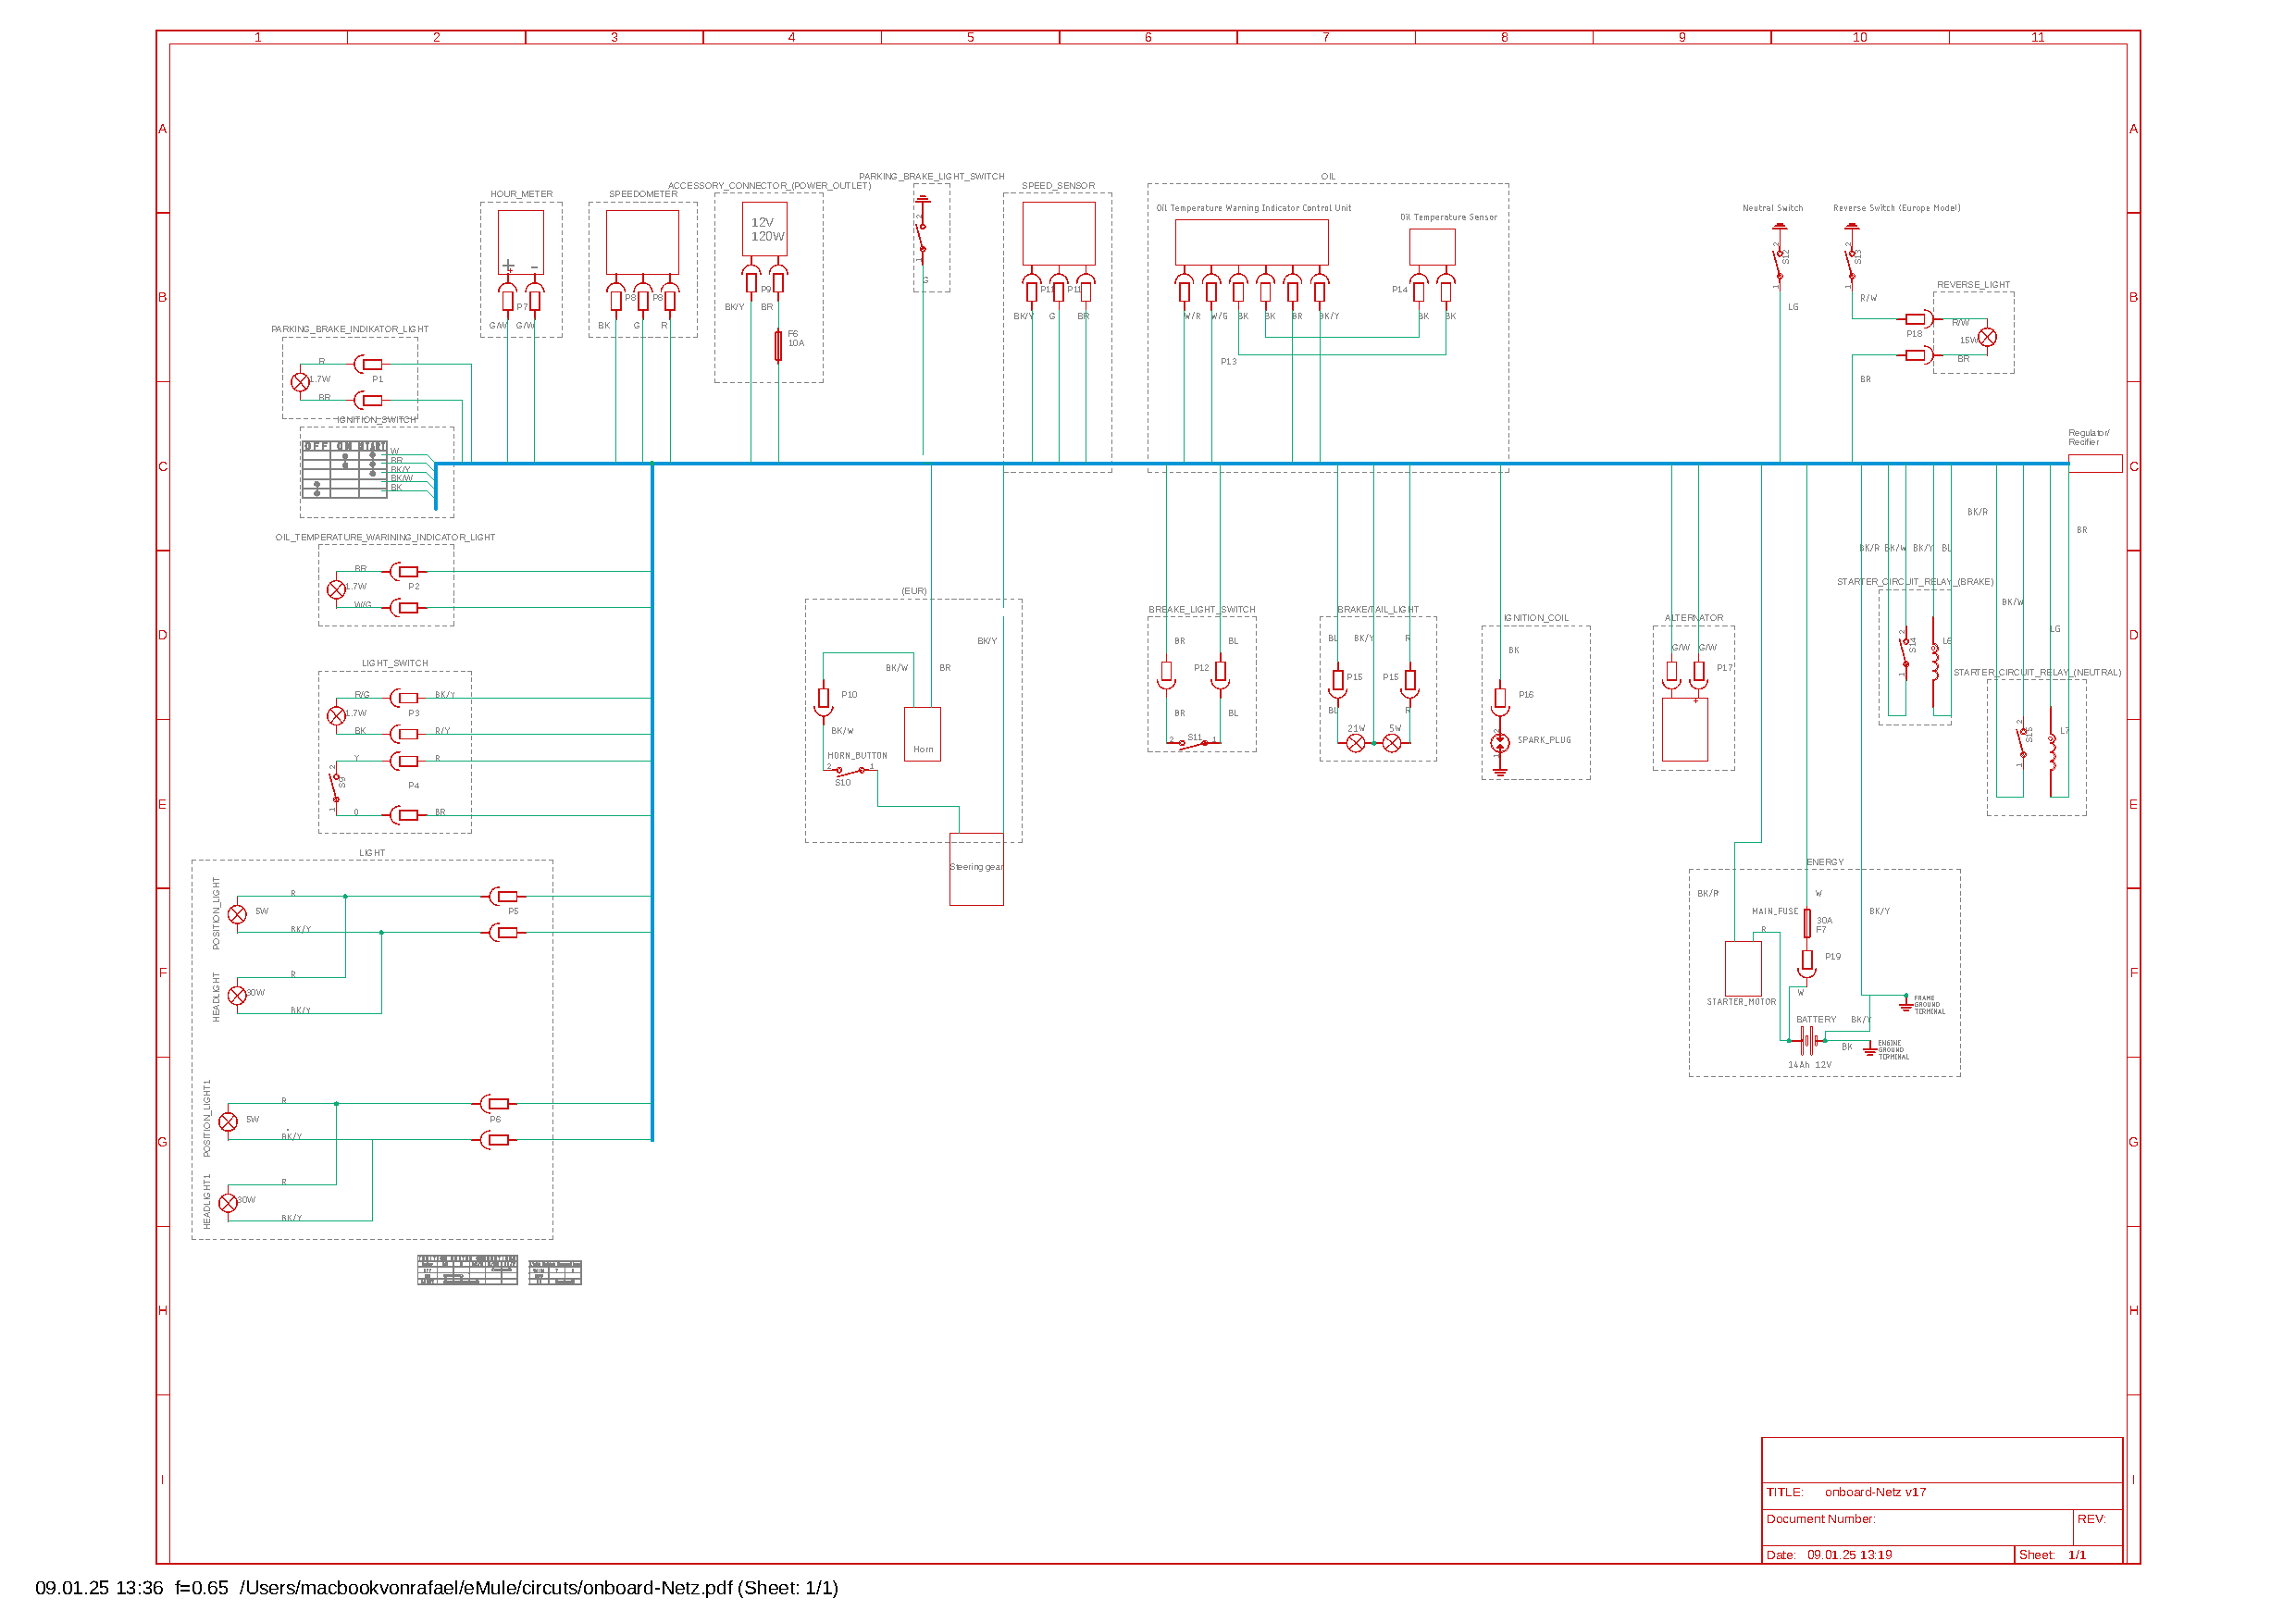
\includepdf[pages=1, fitpaper=true, pagecommand={%
	\thispagestyle{empty} % Entfernt Seitenzahlen und Kopfzeilen
	\begin{center}
		\vspace*{-2cm} % Verschiebt die Caption um 2 cm nach oben
		\captionof{figure}{Schaltplan des LV-Onboard-Netz} % Fügt die Caption ein
		\label{fig:lv_onboard_network} % Für Querverweise
	\end{center}
}]{circuts/onboard-Netz.pdf}
\addtocounter{page}{1} % Seitenzähler korrekt erhöhen

% Vierte PDF: Charger Temperature Control
\subsection{Stromlaufplan Charger Temperature Control}
Für die Erstellung des \textit{Charger Temperature Control} (siehe Abbildung \ref{fig:charger_temperature_control}) Stromlaufplans nach festgelegter Norm und aktuellem Verbaustand wird zunächst eine händische Skizze des Systems, durch die für den Einbau zuständigen Kollegen, angefertigt und an das Dokumentationsteam weitergegeben. Im ersten Schritt wird dieser Stromlaufplan systematisch auf Unstimmigkeiten, wie fehlende Verbindungen oder unklare Symbolik, überprüft. Gefundene Fehler werden im nächsten Schritt markiert und anschließend korrigiert, wobei die Einhaltung elektrotechnischer Standards gewährleistet wird. Zudem erfolgt eine Layoutanpassung zur Verbesserung der Übersichtlichkeit. Im letzten Schritt muss die Normkonformität der Stromlaufplanskizze überprüft werden. Der überarbeitete Stromlaufplan wird abschließend mit Autodesk Fusion 360 in ein DIN-A3-Format übertragen. Dabei werden Titelblock und Legende integriert, um die Professionalität und Lesbarkeit sicherzustellen.

\includepdf[pages=1, fitpaper=true, pagecommand={%
	\thispagestyle{empty} % Entfernt Seitenzahlen und Kopfzeilen
	\begin{center}
		\captionof{figure}{Schaltplan der Charger Temperature Control} % Fügt die Caption ein
		\label{fig:charger_temperature_control} % Für Querverweise
	\end{center}
 }]{circuts/Temperatursteuerung des Ladegerätes.pdf}
\addtocounter{page}{1} % Seitenzähler korrekt erhöhen

% Fünfte PDF: HV-Onboard-Network
\subsection{Stromlaufplan HV-Onboard-Network}
Für die Erstellung des \textit{HV-Onboard-Network} (siehe Abbildung \ref{fig:hv_onboard_network}) Stromlaufplans nach festgelegter Norm und aktuellem Verbaustand wird zunächst eine händische Skizze des Systems, durch die für den Einbau zuständigen Kollegen, angefertigt und an das Dokumentationsteam weitergegeben. Im ersten Schritt wird dieser Stromlaufplan systematisch auf Unstimmigkeiten, wie fehlende Verbindungen oder unklare Symbolik, überprüft. Gefundene Fehler werden im nächsten Schritt markiert und anschließend korrigiert, wobei die Einhaltung elektrotechnischer Standards gewährleistet wird. Zudem erfolgt eine Layoutanpassung zur Verbesserung der Übersichtlichkeit. Im letzten Schritt muss die Normkonformität der Stromlaufplanskizze überprüft werden. Der überarbeitete Stromlaufplan wird abschließend mit Autodesk Fusion 360 in ein DIN-A3-Format übertragen. Dabei werden Titelblock und Legende integriert, um die Professionalität und Lesbarkeit sicherzustellen.

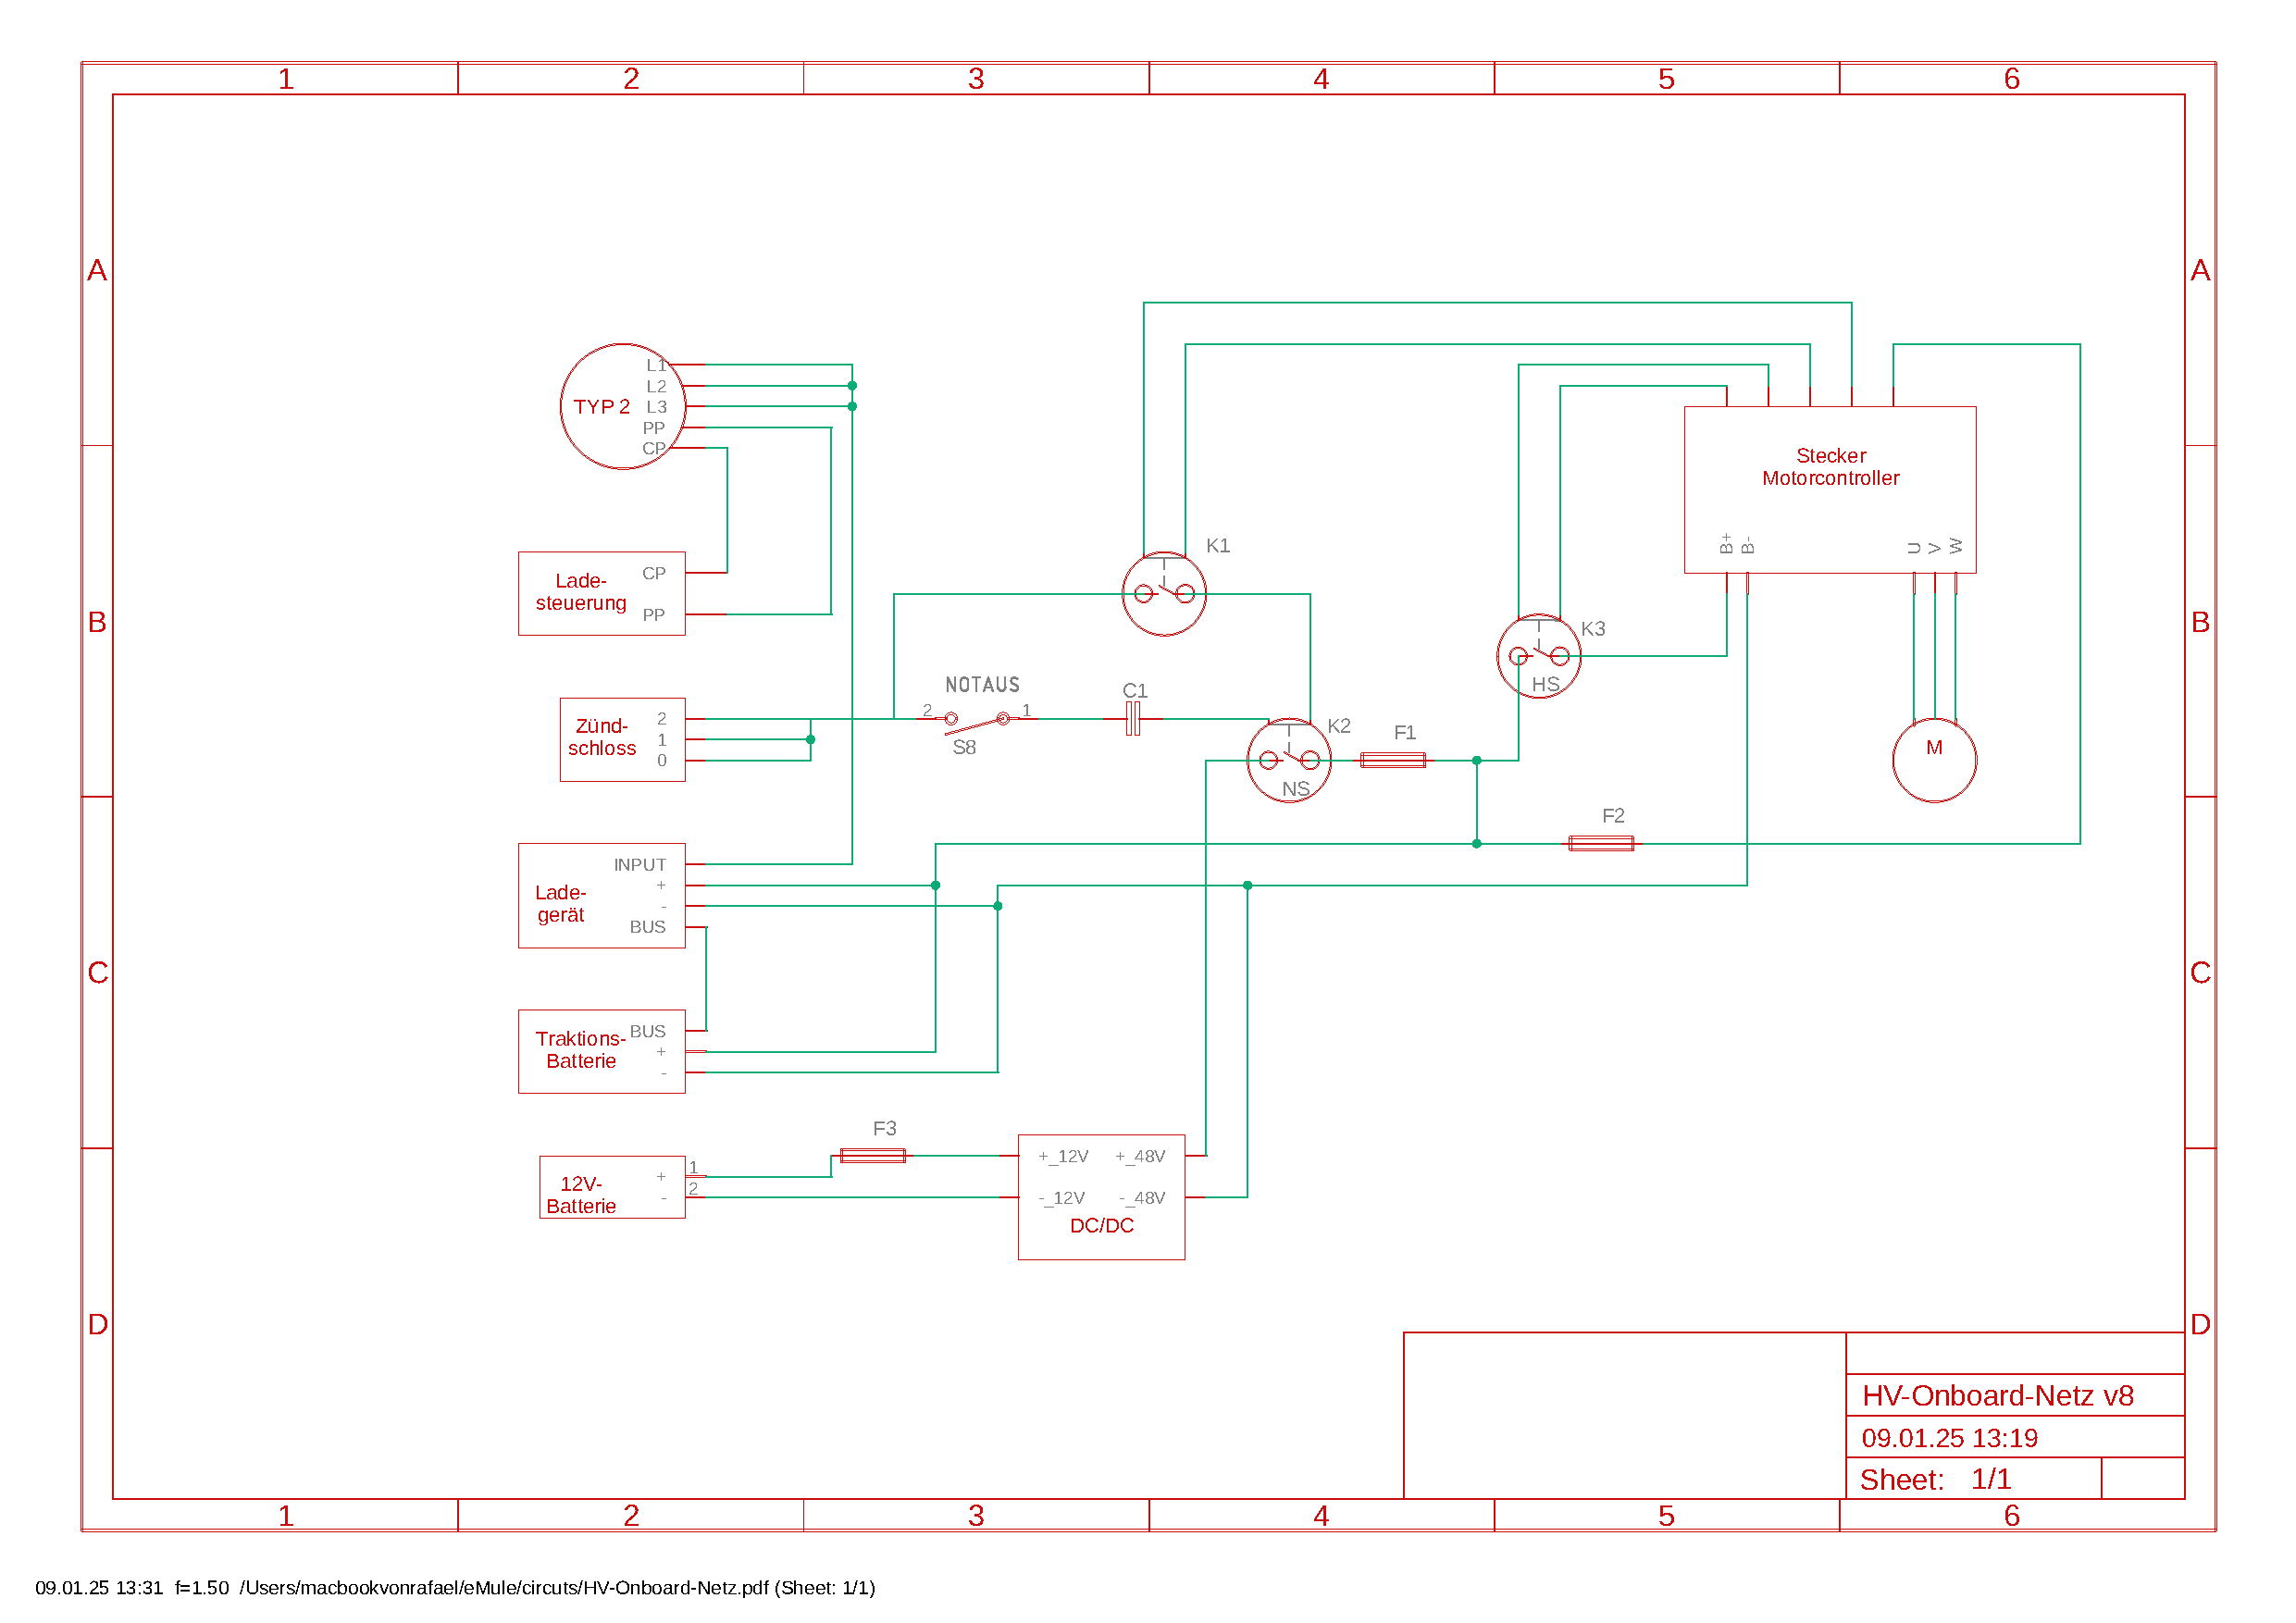
\includepdf[pages=1, fitpaper=true, pagecommand={%
	\thispagestyle{empty} % Entfernt Seitenzahlen und Kopfzeilen
	\begin{center}
		\captionof{figure}{Schaltplan des HV-Onboard-Networks} % Fügt die Caption ein
		\label{fig:hv_onboard_network} % Für Querverweise
	\end{center}
}]{circuts/HV-Onboard-Netz.pdf}
\addtocounter{page}{1}

\section{Legende der Schaltzeichen}
In der folgenden Tabelle (siehe Abbildung \ref{tab:legende}) werden die verwendeten Schaltzeichen des Stromlaufpläne gemäß der Norm DIN EN 60617 erläutert. Diese Schaltzeichen dienen dazu, die elektrischen Komponenten und deren Verbindungen im Stromlaufplan eindeutig und standardisiert darzustellen. Die Legende bietet eine Übersicht über jene Symbole, die in den vorangegangenen Stromlaufplänenplänen verwendet werden, und erleichtert so das Verständnis der Systemarchitektur und Funktionalität der einzelnen Pläne sowie des Gesamtsystems. Dieses Verzeichnis umfasst aktuell:

\begin{multicols}{2}
	\begin{itemize}
		\item Schütz
		\item Kondensator
		\item Funkenstrecke
		\item Masse
		\item Batterie
		\item Sicherung
		\item Schalter
	\end{itemize}
	\columnbreak
	\begin{itemize}
		\item Positive Temperature Coefficient (PTC)-Wiederstand
		\item Potentiometer
		\item Stecker
		\item LED (Light Emitting Diode)
		\item Spule
		\item Drei-Phasen-Motor
	\end{itemize}
\end{multicols}

Im weiteren Verlauf des Projekts kann dieses Verzeichnis beliebig um weitere Schaltzeichen ergänzt und angepasst werden.

\begin{table}[ht]
	\centering
	\resizebox{0.75\textwidth}{!}{% Verkleinert die gesamte Tabelle auf 90 % der Textbreite
		\renewcommand{\arraystretch}{1.8}
		\setlength{\tabcolsep}{15pt}
		\begin{tabular}{|m{5cm}|m{7cm}|}
			\hline
			\textbf{Symbol} & \textbf{Beschreibung} \\
			\hline
			\centering\includegraphics[width=2cm]{Legende/Schütz.png} & \centering Schütz \tabularnewline
			\hline
			\centering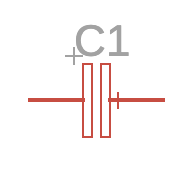
\includegraphics[width=2cm]{Legende/Kondensator.png} & \centering Kondensator \tabularnewline
			\hline
			\centering
\includegraphics[width=2cm]{Legende/Funkenstrecke.png} & \centering Funkenstrecke \tabularnewline
			\hline
			\centering
\includegraphics[width=2cm]{Legende/Ground.png} & \centering Masse (Ground) \tabularnewline
			\hline
			\centering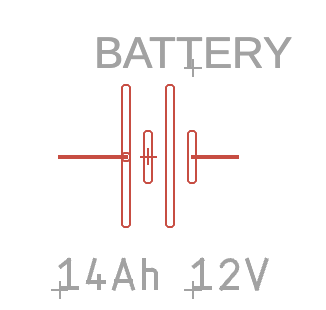
\includegraphics[width=2cm]{Legende/Batterie.png} & \centering Batterie \tabularnewline
			\hline
			\centering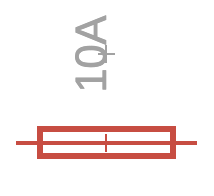
\includegraphics[width=2cm]{Legende/Sicherung.png} & \centering Sicherung \tabularnewline
			\hline
			\centering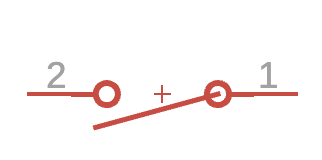
\includegraphics[width=2cm]{Legende/Schalter.png} & \centering Schalter \tabularnewline
			\hline
			\centering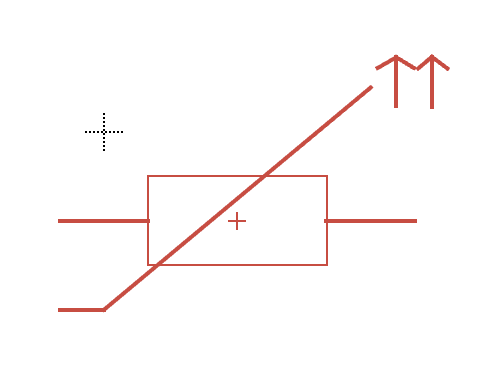
\includegraphics[width=2cm]{Legende/PTC-Widerstand.png} & \centering PTC-Widerstand \tabularnewline
			\hline
			\centering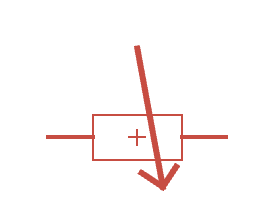
\includegraphics[width=2cm]{Legende/Potentiometer.png} & \centering Potentiometer \tabularnewline
			\hline
			\centering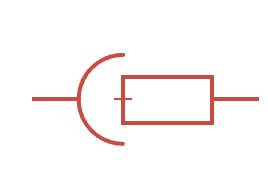
\includegraphics[width=2cm]{Legende/Stecker.png} & \centering Stecker \tabularnewline
			\hline
			\centering
\includegraphics[width=2cm]{Legende/LED.png} & \centering LED \tabularnewline
			\hline
			\centering
\includegraphics[width=2cm]{Legende/Spule.png} & \centering Spule \tabularnewline
			\hline
			\centering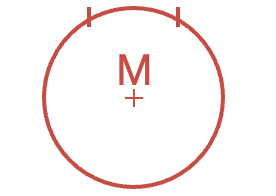
\includegraphics[width=2cm]{Legende/3 Phasen Motor.png} & \centering Drei-Phasen-Motor \tabularnewline
			\hline
	\end{tabular}}
	\caption{Legende der Symbole}
	\label{tab:legende}
\end{table}